\documentclass[a4paper]{scrartcl}
% Use small margins
\usepackage[left=1.5cm, right=1.5cm, top=1cm, bottom=2cm]{geometry}
\usepackage[unicode,
            pdfencoding=auto,
            pdfinfo={
              Title={Sprawozdanie Tranzystor},
              Author={Maciej Mionskowski},
              Subject={Sprawozdanie Tranzystor},
              Keywords={},
              Producer={xelatex},
            },
]{hyperref}
\usepackage[T1]{fontenc}
\usepackage{polski}
\usepackage[polish]{babel}
\usepackage[utf8]{inputenc}
\usepackage{upgreek}
\usepackage{array}
\usepackage{caption}
\usepackage{subcaption}
\usepackage{tabularx}
\usepackage{graphicx}
\usepackage{subfig}
\graphicspath{ {images/} }
\renewcommand{\arraystretch}{1.5}

\author{Maciej Mionskowski}
\title{Sprawozdanie 2}
\date{}
\subtitle{Tranzystor Unipolarny}
\begin{document}
	{\let\newpage\relax\maketitle}
	{\begin{center}Celem ćwiczeń było zapoznanie się z zasadą działania tranzystorów unipolarnych.\end{center}}}
	\begin{section}{Napięcie progowe tranzystora unipolarnego}
		\begin{subsection}{Cel}
			Celem ćwiczenia było wyznaczenie wartości napięcia progowego $ U_{t} $ tranzystora unipolarnego. W tym celu podłączyłem generator sygnału trójkątnego wolno narastającego.

		\end{subsection}
		\begin{subsection}{Analiza}
				\begin{figure}[ht]
				\begin{center}
					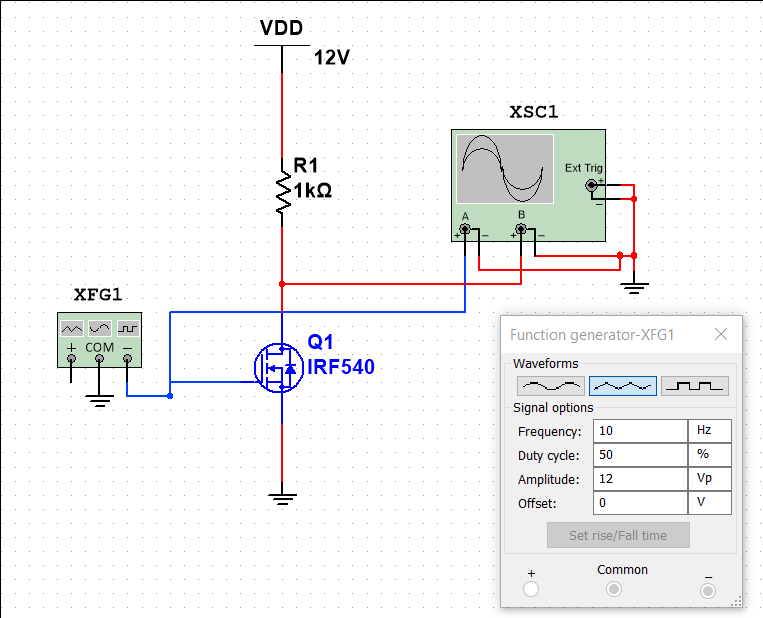
\includegraphics[width=0.8\linewidth]{exercise-1-circuit}
					\caption{Obwód, który posłużył do wyznaczenia napięcia progowego.}
					\label{fig:circuit-1}
				\end{center}
				\end{figure}

				\begin{center}\Huge{$U_{T} = 2.3069V$}\end{center}

				\begin{figure}[ht]
				\begin{center}
					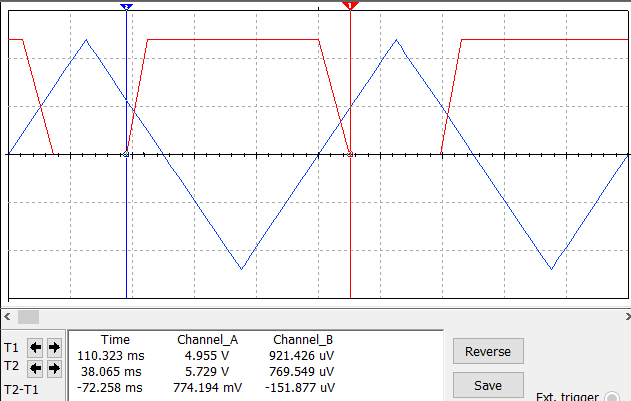
\includegraphics[width=0.7\linewidth]{exercise-1-osciloscope}
					\caption{Pomiar napięcia na bramce i na resystorze w układzie na rysunku \ref{fig:circuit-1}}
					\label{fig:circuit-1-osc}
				\end{center}
				\end{figure}

				\begin{figure}[!ht]
				\begin{center}
					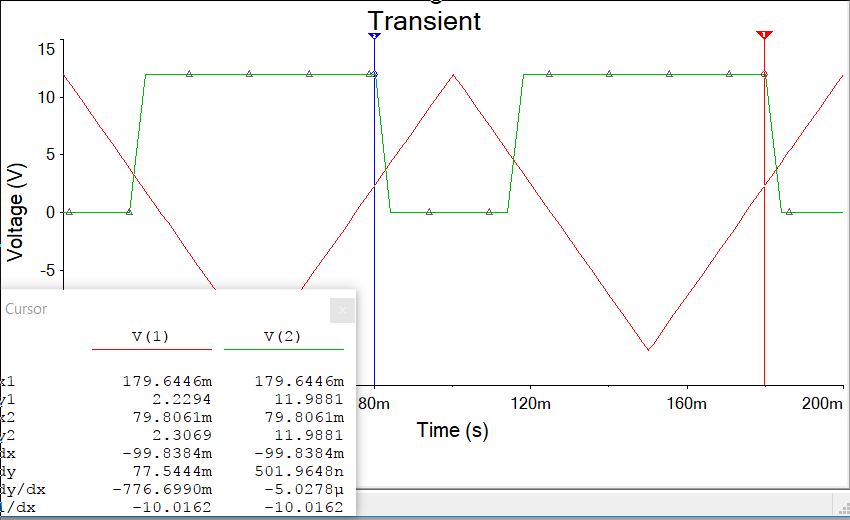
\includegraphics[width=0.7\linewidth,scale=2]{exercise-1-transient}
					\caption{Analiza transient korelacji napięcia na wyjściu generatora (na bramce) $U_{gs}$ do napięcia na rezystorze.}
					\label{fig:circuit-1-transient}
				\end{center}
				\end{figure}
		\end{subsection}
		\begin{subsection}{Wniosek}
			Z powyższej analizy wynika, że tranzystor posiada napięcie progowe wynoszące $\sim0.72 V $. Rozbieżności w powyższych danych spowodowane są błędem pomiarowym polegającym na: niewłaściwym ustawieniu kursorów, a także niedokładności programu MultiSim.
		\end{subsection}
	\end{section}

	\newpage
	\begin{section}{Tranzystor unipolarny w układzie wzmacniacza sygnałów zmiennych}
		\begin{subsection}{Cel}
			Celem ćwiczenia było wyznaczenie wartości rezystora, tak aby układ pracował optymalnie. Doświadczenie wykonałem doświadczalnie poprzez zastosowanie potencjometrów, analizy transient i oscyloskopa. Ponadto należało pokazać i poznać zasadę działania takiego układu jako wzmacniacza sygnału zmiennego.
		\end{subsection}

		\begin{subsection}{Analiza}
				\begin{figure}[!ht]
				\begin{center}
					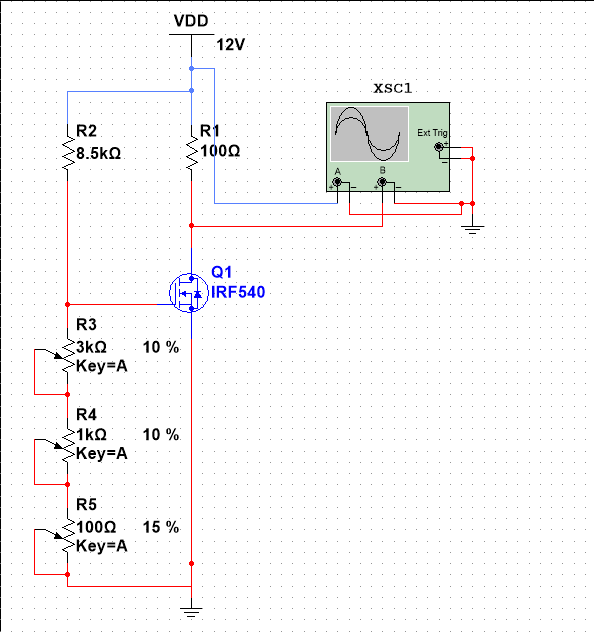
\includegraphics[width=0.5\linewidth,scale=2]{exercise-2-circuit-pre-change}
					\caption{Prosty obwód z tranzystorem NMOS do eksperymentalnego wyznaczenia rezystancji $ R $}
					\label{fig:circuit-2-circuit-pre-change}
				\end{center}

				\end{figure}
				\begin{figure}[!ht]
				\begin{center}
					\begin{subfigure}{.45\textwidth}
						\begin{center}
						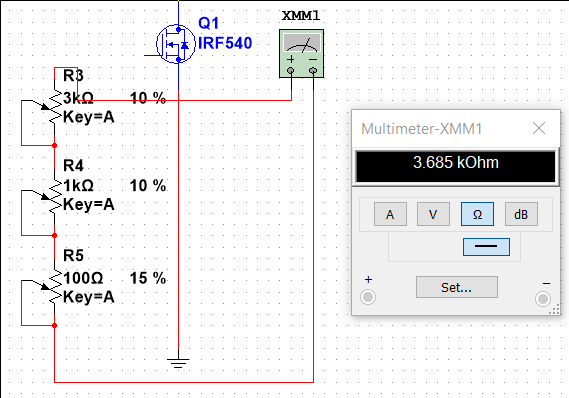
\includegraphics[width=\linewidth,scale=2]{exercise-2-ohms}
						\caption{Pomiar na omomierzu dla rezystora zastępczego, którego wartość została wyznaczona doświadczalnie}
						\label{fig:exercise-2-punkt-pracy}
						\end{center}
					\end{subfigure}
					\begin{subfigure}{.45\textwidth}
						\begin{center}
						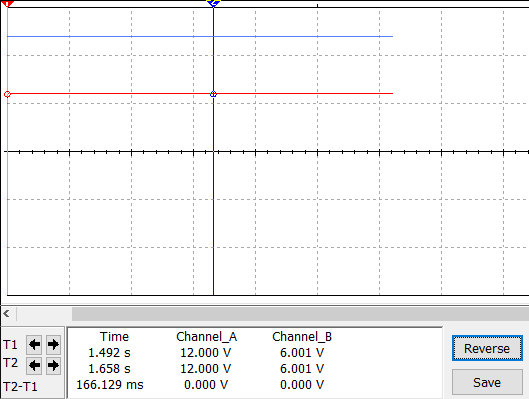
\includegraphics[width=\linewidth,scale=2]{exercise-2-punkt-pracy}
						\caption{Pomiar napięcia $U_{wy}$ na oscyloskopie dla $ R_{Z} = 3.685k\Omega $}
						\label{fig:exercise-2-punkt-pracy}
						\end{center}
					\end{subfigure}
				\end{center}
				\caption{Pomiary napięcia i rezystancji wykonane w celu wyznaczenia rezystancji zastępczej.}
				\end{figure}

				\begin{figure}[!ht]
					\begin{center}
						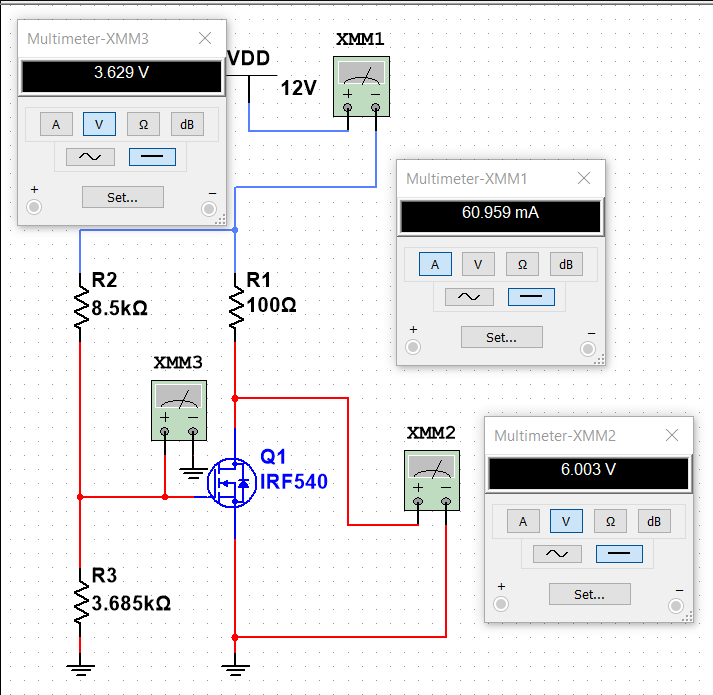
\includegraphics[width=.6\linewidth]{exercise-2-pomiary}
						\caption{Pomiary punktu pracy i napięcia na bramce wykonane w obwodzie po zastąpieniu potencjometrów rezystorem o rezystancji zastępczej $R_{z}$}
					\end{center}
				\end{figure}

				\begin{table}[!ht]
					\begin{center}
					\caption{Wartości zmierzone w obwodzie na rysunku \ref{fig:circuit-2-circuit-pre-change} }
					\begin{tabular}{| l | l | l | l | l | l | l | l |}
						\hline
						$ U_{DD} $ & $ R_{D} $ & $ U_{GS} $ & $ U_{DS} $ & $ I_{D} $ & $(U_{DS}, I_{D} )$ & $ k_{u} $ & $ g_{m} $ \\ \hline
					
						$ 12V $ & $ 100 \Omega $ & $ 3.629V $ & $ 6.003 V $ & $ 61 mA$ & $ 6.003 V, 61 mA $ & $ \frac{1}{2} $ & $ 16.8mS$ \\ \hline
					\end{tabular}
					\end{center}
				\end{table}
				\begin{figure}[!ht]
						\begin{center}
							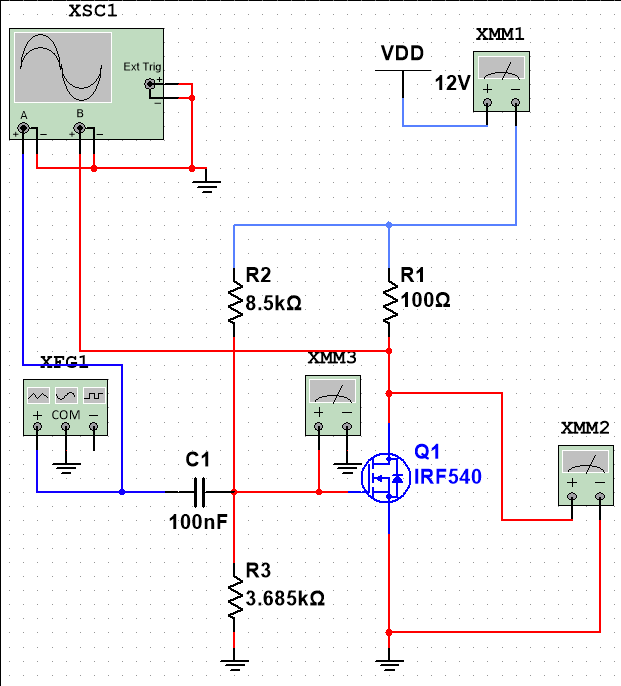
\includegraphics[width=0.4\linewidth,scale=2]{exercise-2-sin-amp-circuit}
							\caption{Obwód z podłączonym generatorem prądu zmiennego.}
							\label{fig:circuit-2-circuit-amp-circ}
						\end{center}
				\end{figure}
				\begin{figure}[!ht]
						\begin{center}
							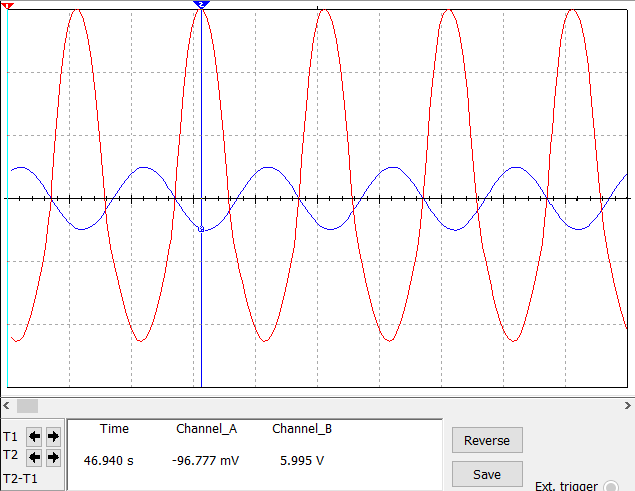
\includegraphics[width=0.6\linewidth,scale=2]{exercise-2-wzmocnienie-sin}
							\caption{Pomiar wzmocnienia sygnału wejściowego. Należy zwrócić uwagę na skalę (wartości na dole)}
							\label{fig:circuit-2-circuit-amp}
						\end{center}
				\end{figure}
		\end{subsection}
		\pagebreak
		\begin{subsection}{Wniosek}
			Tranzystor w układzie polaryzacyjnym może być użyty jako wzmacniacz sygnału zmiennego. Doświadczalne wyznaczanie rezystancji zastępczej jest dość efektywnym sposobem osiągnięcia tego samego rezultatu mniejszym nakładem kognitywnym. Wartości w tabeli zgadzają się z informacjami teoretycznymi przekazanymi na wykładzie. Optymalne wartości pracy tranzystora wyznaczają wzory: $ U_{wy} = \frac{1}{2}U_{DD} $, $ I_{D} = \frac{U_{DD} - U_{wy}}{R_{D}} $.
		\end{subsection}
	\end{section}
	\begin{section}{Tranzystor unipolarny CMOS jako klucz przełączający}

		\begin{subsection}{Cel}
			Celem ćwiczenia było poznanie zasady działania tranzystora unipolarnego CMOS jako klucza przełączającego oraz zmierzenie czasów włączenia i wyłączenia tranzystora.
		\end{subsection}
		\begin{subsection}{Analiza}
				\begin{figure}[ht]
				\begin{center}
					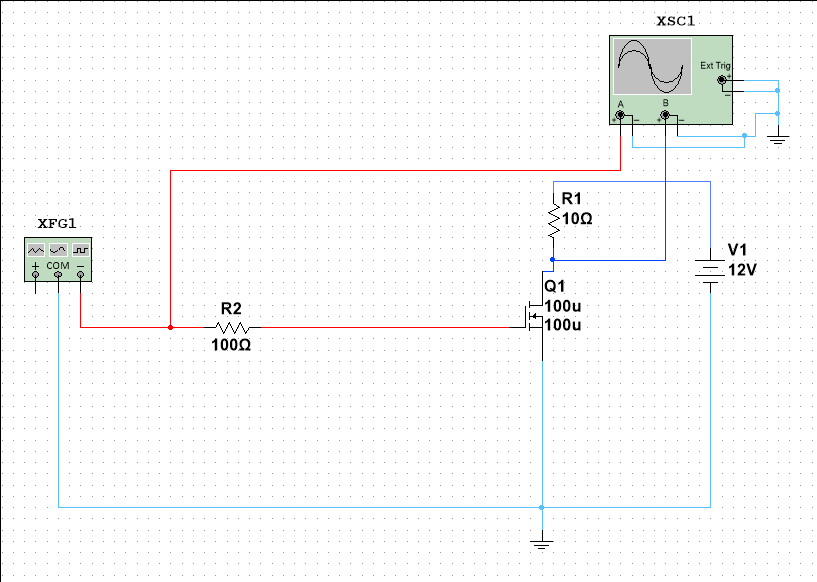
\includegraphics[width=0.5\linewidth,scale=2]{exercise-5-circuit}
					\caption{Prosty obwód z tranzystorem unipolarnym użytym jako klucz.}
					\label{fig:circuit-3}
				\end{center}
				\end{figure}
		\end{subsection}
		\begin{subsection}{Wniosek}
		\end{subsection}
	\end{section}
	\begin{section}{Klucz przełączający - wstęp do układów logicznych}
		\begin{subsection}{Cel}
			Celem ćwiczenia było zapoznanie się z zasadą działania układów logicznych (stan niski, wysoki). Pomiar napięć, poznanie różnic między tranzystorami P i N.
		\end{subsection}
		\begin{subsection}{Analiza}
				\begin{figure}[ht]
				\begin{center}
					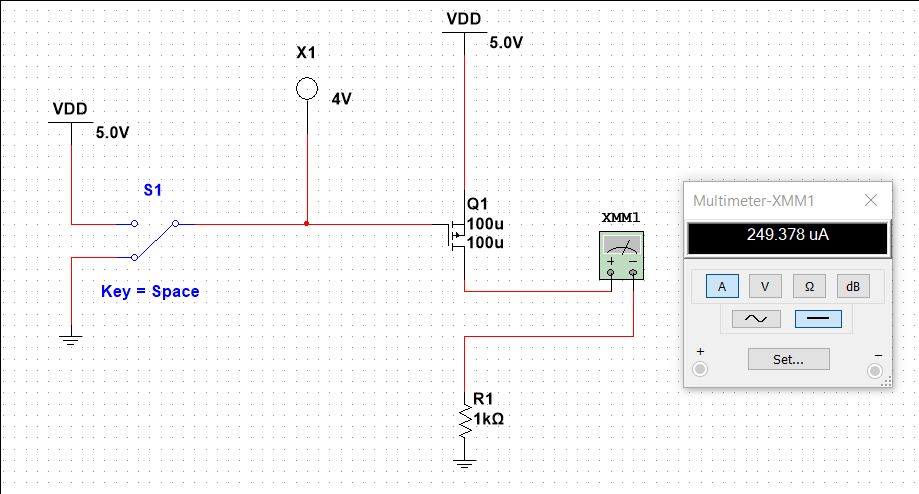
\includegraphics[width=0.65\linewidth]{exercise-6-tranzystor-wstep-circuit-pmos-on}
					\caption{Klucz przełączający z tranzystorem PMOS, stan włączony}
					\label{fig:circuit-4-p-on}
				\end{center}
				\end{figure}
				\begin{figure}[!ht]
				\begin{center}
					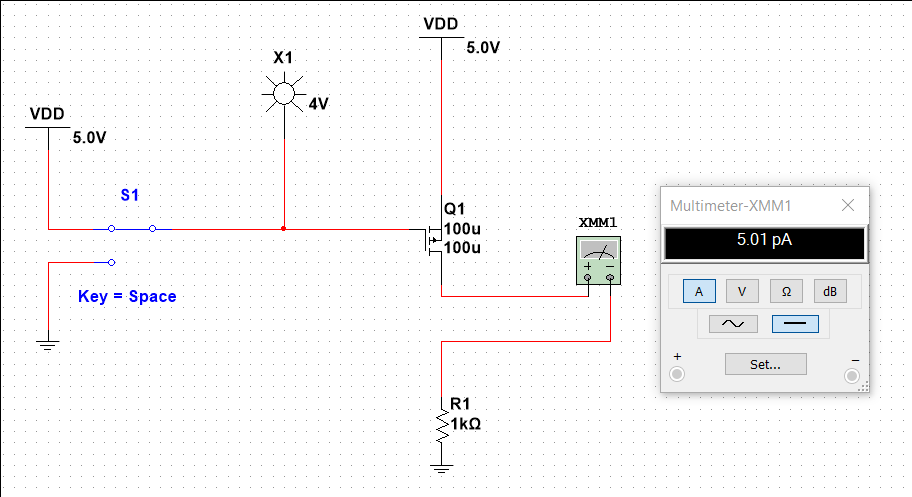
\includegraphics[width=0.65\linewidth]{exercise-6-tranzystor-wstep-circuit-pmos-off}
					\caption{Klucz przełączający z tranzystorem PMOS, stan wyłączony}
					\label{fig:circuit-4-p-off}
				\end{center}
				\end{figure}
				\begin{table}[!ht]
					\begin{center}
					\caption{Tabela prawdy dla klucza przełączającego z tranzystorem PMOS}
					\begin{tabular}{| l | l |}
						\hline
						Sygnał na bramce tranzystora & stan tranzystora PMOS \\\hline
						1 & wyłączony \\ \hline
						0 & włączony \\ \hline
					\end{tabular}
					\end{center}
				\end{table}
				\begin{figure}[!ht]
				\begin{center}
					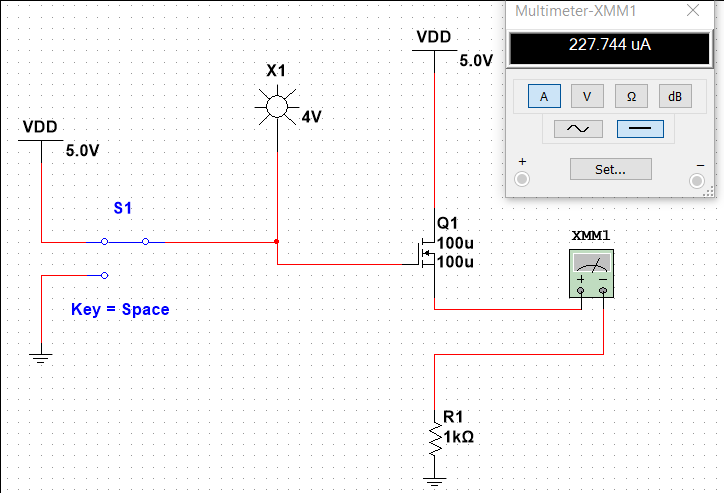
\includegraphics[width=0.65\linewidth]{exercise-6-tranzystor-wstep-circuit-nmos-on}
					\caption{Klucz przełączający z tranzystorem NMOS, stan włączony}
					\label{fig:circuit-4-n-on}
				\end{center}
				\end{figure}
				\begin{figure}[!ht]
				\begin{center}
					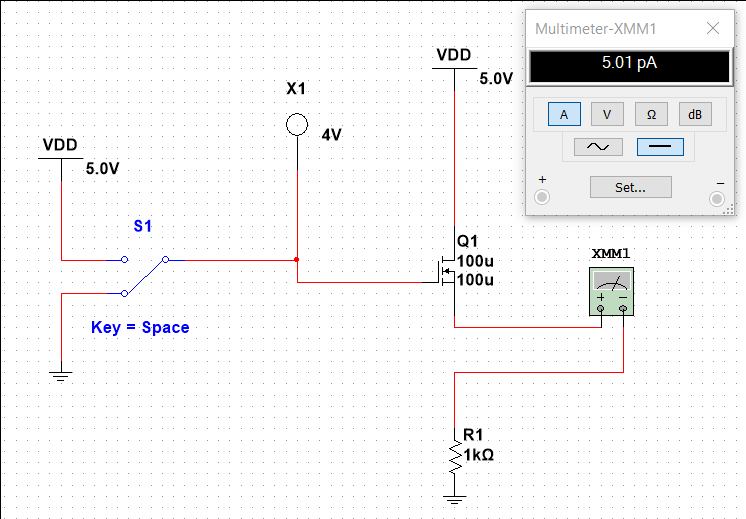
\includegraphics[width=0.65\linewidth]{exercise-6-tranzystor-wstep-circuit-nmos-off}
					\caption{Klucz przełączający z tranzystorem NMOS, stan wyłączony}
					\label{fig:circuit-4-n-off}
				\end{center}
				\end{figure}
				\begin{table}[!ht]
					\begin{center}
					\caption{Tabela prawdy dla klucza przełączającego z tranzystorem NMOS}
					\begin{tabular}{| l | l |}
						\hline
						Sygnał na bramce tranzystora & stan tranzystora NMOS \\\hline
						1 & włączony \\ \hline
						0 & wyłączony \\ \hline
					\end{tabular}
					\end{center}
				\end{table}

				\pagebreak
		\end{subsection}
		\pagebreak
		\begin{subsection}{Wniosek}
			Tranzystor może być użyty jako klucz przełączający. Podanie sygnału wysokiego na bramkę tranzystora NMOS aktywuje klucz, analogicznie podanie sygnału niskiego na bramkę tranzystora PMOS również aktywuje/zamyka klucz.
		\end{subsection}
	\end{section}
	\begin{section}{Inwerter logiczny CMOS - NOT}
		\begin{subsection}{Cel}
			Celem doświadczenia było zapoznanie z zasadą działania inwertera logicznego CMOS - NOT.
		\end{subsection}
		\begin{subsection}{Analiza}
				\begin{figure}[ht]
				\begin{center}
					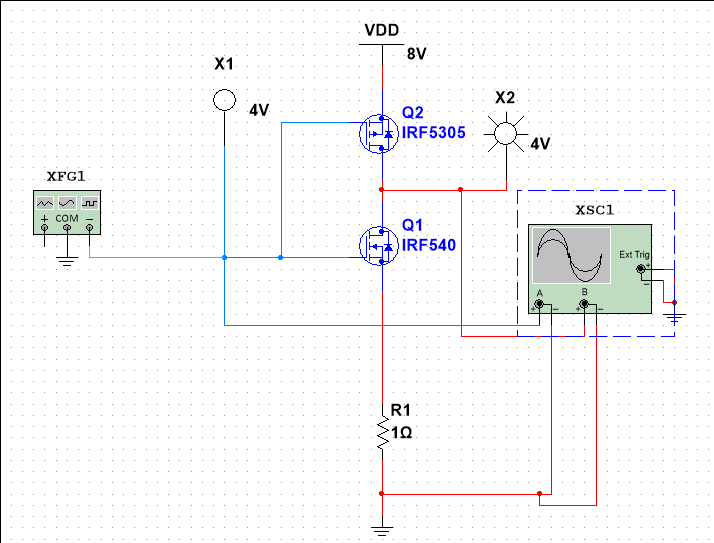
\includegraphics[width=0.5\linewidth]{exercise-7-inwerter-circuit}
					\caption{Inwerter CMOS}
					\label{fig:circuit-7-cmos}
				\end{center}
				\end{figure}
				\begin{figure}[ht]
				\begin{center}
					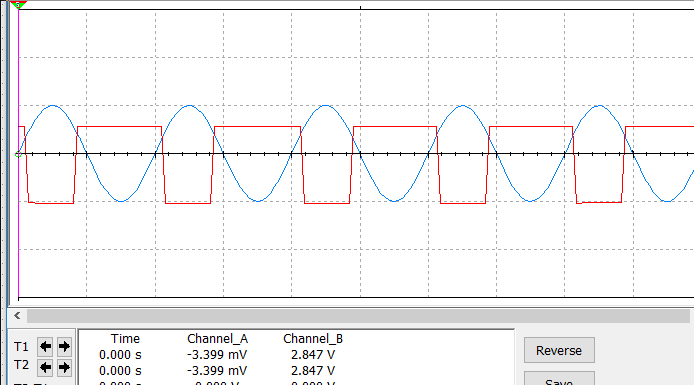
\includegraphics[width=0.5\linewidth]{exercise-7-inwerter-osciloscope}
					\caption{Zależność stanu logicznego wyjścia od wejścia w bramce NOT}
					\label{fig:circuit-7-cmos}
				\end{center}
				\end{figure}
				\begin{table}[!ht]
					\begin{center}
					\caption{Tabela prawdy dla inwertera logicznego NOT}
					\begin{tabular}{| l | l | l | l |}
						\hline
						Wejście & Wyjście & Q1 & Q2 \\\hline
						1 & 0 & 1 & 0 \\ \hline
						0 & 1 & 0 & 1 \\ \hline
					\end{tabular}
					\end{center}
				\end{table}
		\end{subsection}
		\begin{subsection}{Wniosek}
			Inwerter logiczny CMOS - NOT odwraca stan sygnału. Jest to bardzo prosta bramka logiczna, za pomocą której można budować inne bramki. Do budowy stosujemy dwa komplementarne tranzystory tak aby w zależności od sygnału wejściowego raz jeden był otwarty, a raz drugi.
		\end{subsection}
	\end{section}
	\begin{section}{Bramka NAND w technologii CMOS}
		\begin{subsection}{Cel}
			Celem doświadczenia było zapoznanie z budowią i zasadą działania bramki NAND.
		\end{subsection}
		\begin{subsection}{Analiza}
				\begin{figure}[ht]
				\begin{center}
					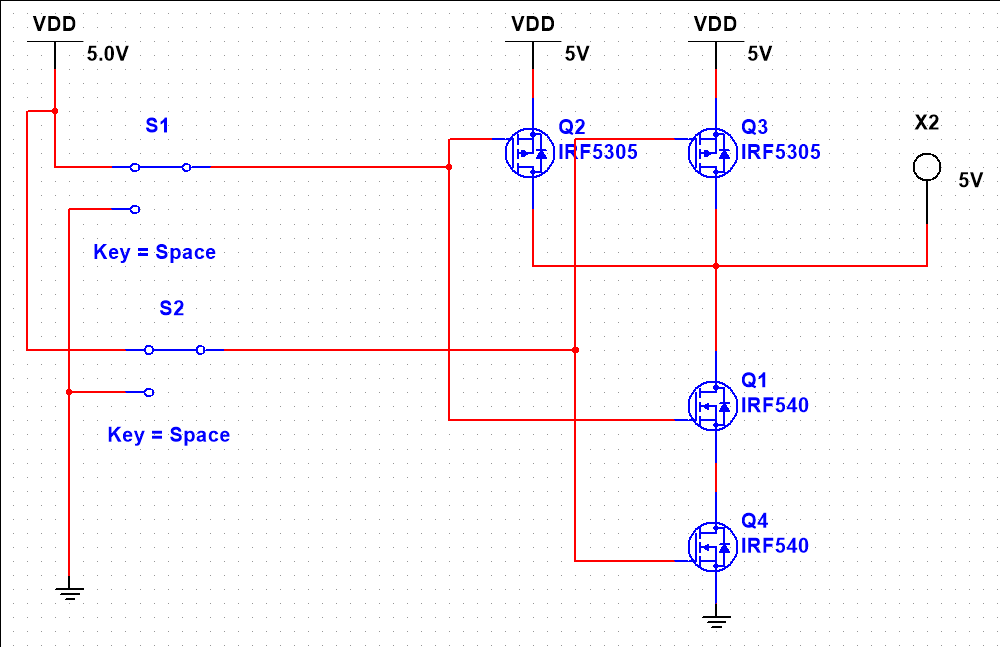
\includegraphics[width=0.7\linewidth]{exercise-8-nand-gate}
					\caption{Bramka NAND - 2 tranzystory PMOS połączone równolegle i 2 NMOS połączone szeregowo}
					\label{fig:circuit-7-cmos}
				\end{center}
				\end{figure}
				\begin{table}[!ht]
					\begin{center}
					\caption{Tabela prawdy dla bramki NAND}
					\begin{tabular}{| l | l | l | l | l | l | l |}
						\hline
						S1 & S2 & Wyjście & Q2 & Q3 & Q1 & Q4 \\\hline
						1 & 1 & 0 & 0 & 0 & 1 & 1 \\ \hline
						0 & 1 & 1 & 1 & 0 & 0 & 1 \\ \hline
						1 & 0 & 1 & 0 & 1 & 1 & 0 \\ \hline
						0 & 0 & 1 & 1 & 1 & 0 & 0 \\ \hline
					\end{tabular}
					\end{center}
				\end{table}
		\end{subsection}
		\begin{subsection}{Wniosek}
			Bramka logiczna NAND - NOT AND (analogiczna do koniunkcji w logice klasycznej) działa na zasadzie "połączenia" funkcji 'i' i 'lub'. W jednym momencie włączone są jedynie dwa tranzystory, powoduje to, że prąd nie może płynąć bezpośrednio od $ V_{DD} $ do masy.
		\end{subsection}
	\end{section}
	\clearpage
	\begin{section}{Bramka AND w technologii CMOS}
		\begin{subsection}{Cel}
			Celem doświadczenia było zapoznanie z budową i zasadą działania bramki AND.
		\end{subsection}
		\begin{subsection}{Analiza}
				\begin{figure}[ht]
				\begin{center}
					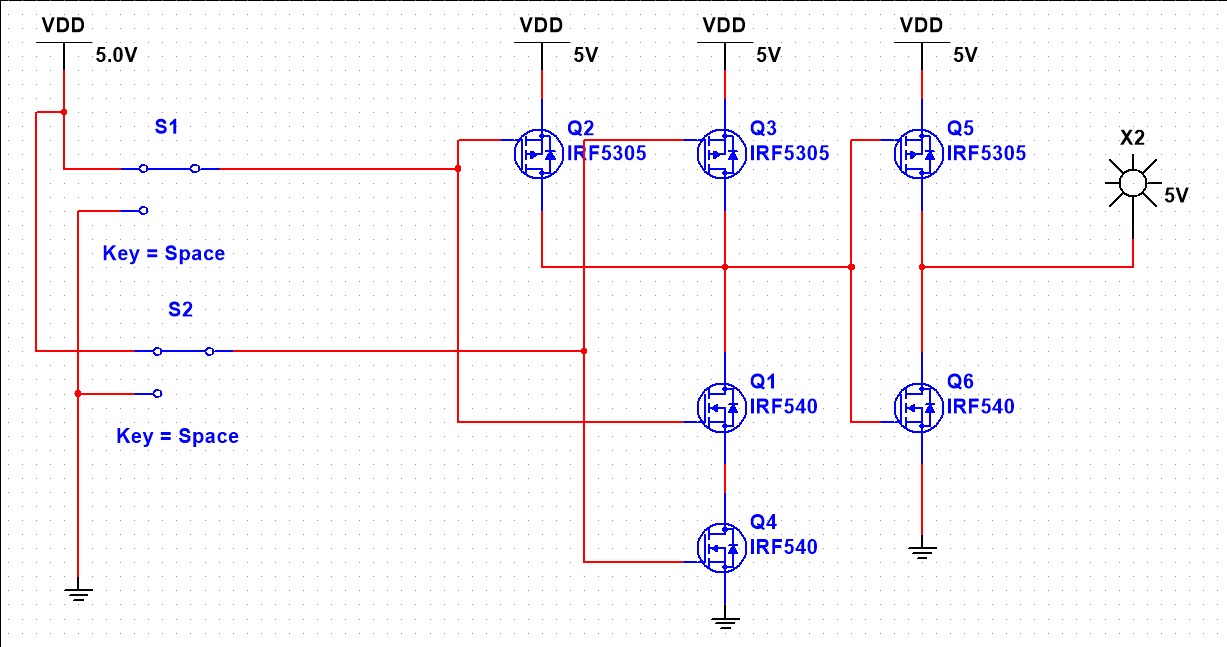
\includegraphics[width=0.8\linewidth]{exercise-9-and-gate-circuit}
					\caption{Bramka AND - 2 tranzystory PMOS połączone równolegle i 2 NMOS połączone szeregowo + 2 na inwerter}
					\label{fig:circuit-7-cmos}
				\end{center}
				\end{figure}
				\begin{table}[!ht]
					\begin{center}
					\caption{Tabela prawdy dla bramki AND - 2 tranzystory PMOS połączone równolegle i 2 NMOS połączone szeregowo + 2 komplementarne na inweter}
					\begin{tabular}{| l | l | l | l | l | l | l | l | l |}
						\hline
						S1 & S2 & Wyjście & Q2 & Q3 & Q1 & Q4 & Q5 & Q6 \\\hline
						1 & 1 & 1 & 0 & 0 & 1 & 1 & 1 & 0 \\ \hline
						0 & 1 & 0 & 1 & 0 & 0 & 1 & 0 & 1 \\ \hline
						1 & 0 & 0 & 0 & 1 & 1 & 0 & 0 & 1 \\ \hline
						0 & 0 & 0 & 1 & 1 & 0 & 0 & 0 & 1 \\ \hline
					\end{tabular}
					\end{center}
				\end{table}
		\end{subsection}
		\begin{subsection}{Wniosek}
			Bramka logiczna AND lub w tym przypadku NOT NAND działa na zasadzie "połączenia" bramek 'i', 'lub' i negacji W jednym momencie włączone są jedynie dwa tranzystory (wykluczając inwerter), powoduje to, że prąd nie może płynąć bezpośrednio od $ V_{DD} $ do masy.
		\end{subsection}
	\end{section}
	\clearpage
	\begin{section}{Bramka NOR w technologii CMOS}
		\begin{subsection}{Cel}
			Celem doświadczenia było zapoznanie z budową i zasadą działania bramki NOR.
		\end{subsection}
		\begin{subsection}{Analiza}
				\begin{figure}[ht]
				\begin{center}
					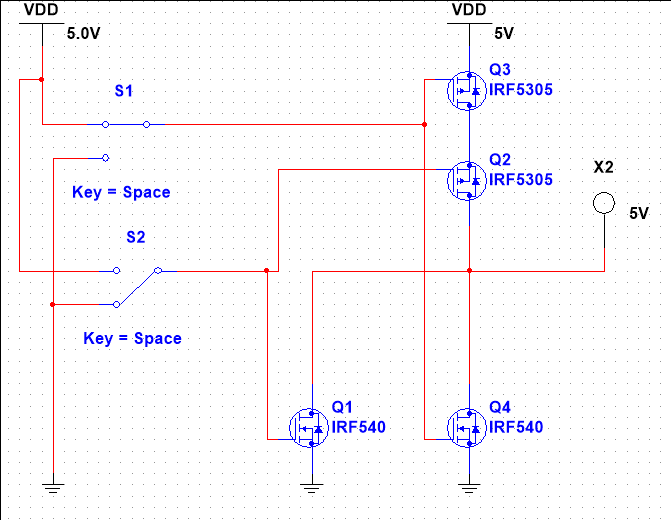
\includegraphics[width=0.8\linewidth]{exercise-10-nor-circuit}
					\caption{Bramka NOR - 2 tranzystory NMOS połączone równolegle i 2 PMOS połączone szeregowo }
					\label{fig:circuit-7-cmos}
				\end{center}
				\end{figure}
				\begin{table}[!ht]
					\begin{center}
					\caption{Tabela prawdy dla bramki NOR}
					\begin{tabular}{| l | l | l | l | l | l | l | l | l |}
						\hline
						S1 & S2 & Wyjście & Q3 & Q2 & Q1 & Q4 \\\hline
						1 & 1 & 0 & 0 & 0 & 1 & 1 \\ \hline
						0 & 1 & 0 & 1 & 0 & 1 & 0 \\ \hline
						1 & 0 & 0 & 0 & 1 & 0 & 1 \\ \hline
						0 & 0 & 1 & 1 & 1 & 0 & 0 \\ \hline
					\end{tabular}
					\end{center}
				\end{table}
		\end{subsection}
		\begin{subsection}{Wniosek}
			Bramka logiczna NOR - NOT OR jest analogiczna do negacji alternatywy w logice klasycznej. W jednym momencie włączone są jedynie dwa tranzystory, powoduje to, że prąd nie może płynąć bezpośrednio od $ V_{DD} $ do masy.
		\end{subsection}
	\end{section}
	\clearpage
	\begin{section}{Bramka OR w technologii CMOS}
		\begin{subsection}{Cel}
			Celem doświadczenia było zapoznanie z budową i zasadą działania bramki OR.
		\end{subsection}
		\begin{subsection}{Analiza}
				\begin{figure}[ht]
				\begin{center}
					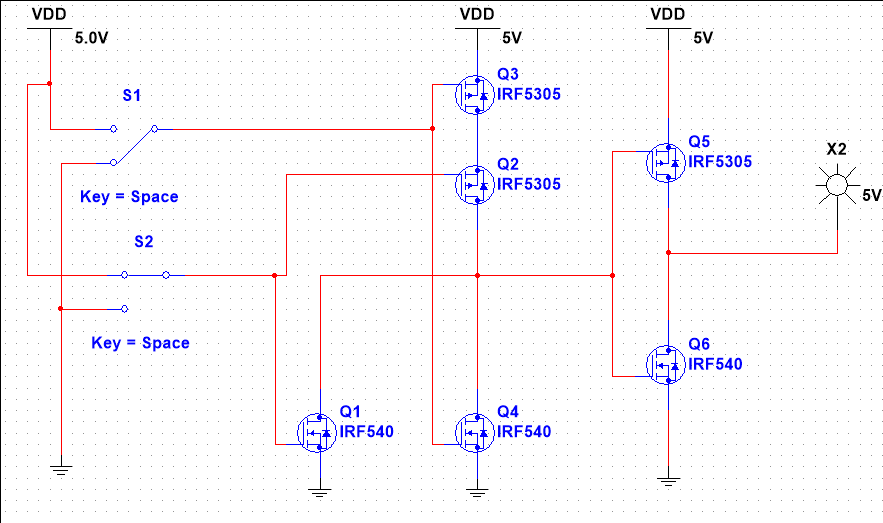
\includegraphics[width=0.8\linewidth]{exercise-11-or-circuit}
					\caption{Bramka OR - 2 tranzystory NMOS połączone równolegle i 2 PMOS połączone szeregowo + 2 na inwerter}
					\label{fig:circuit-7-cmos}
				\end{center}
				\end{figure}
				\begin{table}[!ht]
					\begin{center}
					\caption{Tabela prawdy dla bramki OR}
					\begin{tabular}{| l | l | l | l | l | l | l | l | l |}
						\hline
						S1 & S2 & Wyjście & Q2 & Q3 & Q1 & Q4 & Q5 & Q6 \\\hline
						1 & 1 & 1 & 0 & 0 & 1 & 1 & 1 & 0 \\ \hline
						0 & 1 & 1 & 1 & 0 & 1 & 0 & 1 & 0 \\ \hline
						1 & 0 & 1 & 0 & 1 & 0 & 1 & 1 & 0 \\ \hline
						0 & 0 & 0 & 1 & 1 & 0 & 0 & 0 & 1 \\ \hline
					\end{tabular}
					\end{center}
				\end{table}
		\end{subsection}
		\begin{subsection}{Wniosek}
			Bramka logiczna OR, lub w tym przypadku NOT NOR jest analogiczna do alternatywy w logice klasycznej. W jednym momencie włączone są jedynie dwa tranzystory (wykluczając inwerter), powoduje to, że prąd nie może płynąć bezpośrednio od $ V_{DD} $ do masy.
		\end{subsection}
	\end{section}
\end{document}
